% !TeX root = ./main.tex
\documentclass[main]{subfiles}
\begin{document}
\chapter{Криволинейные интегралы}

\section{Спрямляемые кривые}
 \begin{definition}
     Пусть $\Gamma:[a,b]\rightarrow {\vR^n},\ n\geq 2$ - отображение, предполагаем $\Gamma\in C([a,b])$ и отображение $\Gamma$ инъективно.\\
      \textbf{Разомкнутой кривой} далее в зависимости от контекста будем называть и отображение $\Gamma(\cdot),$ и образ $\Gamma([a,b])$. 
      Если $\Gamma(a)=\Gamma(b),$ но отображение $\Gamma$ инъективно на $[a,b),$ то отображение $\Gamma(\cdot)$ или образ $\Gamma([a,b])$
       далее будем называть \textbf{замкнутой кривой}. \\ Разомкнутую или замкнутую кривую далее называем \textbf{кривой}. 
       Если $\Gamma$ - разомкнутая кривая, то её концами будем называть точки $\Gamma(a)$ и $\Gamma(b)$, 
       при этом также $\Gamma(a)$ будем называть \textbf{началом} $\Gamma(\cdot),$ а $\Gamma(b)$ - 
       \textbf{конец} $\Gamma(\cdot).$ Если $\{ t_k\}^n_{k=0}$ - разбиение отрезка
        $[a,b], a=t_0<t_1<\dots<t_n=b,$ то множество $\{ \Gamma(t_k)\}_{k=0}^n$ назовём \textbf{разбиением кривой} $\Gamma(\cdot)$.
 \end{definition}
    
 
 \subsubsection{Определение спрямляемой кривой}
 Пусть $\{ \Gamma(t_k)\}^n_{k=0}$ - разбиение кривой $\Gamma$, положим
 \[ l(\{\Gamma(t_k)\}^n_{k=0})\stackrel{def}{=}\sum\limits_{k=0}^{n-1}|| \Gamma(t_{k+1})-\Gamma(t_k)||_{\vR^n} \tag{1} \]
 \[ l(\Gamma(\cdot))\overset{def}{=}sup\ l(\{\Gamma(t_k)\}^n_{k=0}) \tag{2} \]
 где в правой части (2) $sup$ берётся по всем разбиениям кривой $\Gamma(\cdot).$\\
 Если $l(\Gamma(\cdot))<\infty$, то кривая $\Gamma(\cdot)$ называется \textbf{спрямлемой}, а величина $l(\Gamma(\cdot))$ называется \textbf{длиной кривой $\Gamma(\cdot)$}
 \subsubsection{Свойства спрямляемых кривых}
 1. $|| \Gamma(b)-\Gamma(a)||_{\vR^n}\leq l(\Gamma(\cdot))$ - доказательство следует из того, что разбиение $\{ t_k\}^1_{k=0},\ t_0=a<b=t,$ участвует во множестве разбиений.\\
 2. Пусть $a<c<b$, кривая $\Gamma([a,b])$ спрямляема; \\
  тогда \[l(\Gamma([a,b]))=l(\Gamma([a,c]))+l(\Gamma([c,b]))\tag{3}\]
  (3) следует из того, что, не умаляя общности можно считать $c\in \{t_k\}^n_{k=0},$ тогда\\ \( l(\{\Gamma(t_k)^m_{k=0}\})+l(\{\Gamma(t_k)\}^n_{k=m})=l(\{\Gamma(t_k)\}^n_{k=0}), \) если $c=t_m,$ и далее перейти к супремуму в левой и правой части.\\
3. Пусть $a<c<b,$ тогда $l(\Gamma[a,c])<l(\Gamma[a,b])$
 \begin{proof}
Для доказательства для $\forall$ разбиения $\{\Gamma(t_k)\}_{k=0}^m,$ $t_m=c,$ рассмотрим разбиение $\{ \Gamma(t_k)\}^{m+1}_{k=0}, t_{m+1}=b,$ тогда\\
 $l(\{\Gamma(t_k)\}^{m+1}_{k=0})=l(\{\Gamma(t_k)\}^m_{k=0})+||\Gamma(t_{m+1})-
 \Gamma(t_m)||_{{\vR^n}}=l(\{\Gamma(t_k)\}^m_{k=0})+||\Gamma(b)-\Gamma(c)||_{\vR^n},$ поэтому 
 \[l(\Gamma([a,b]))\geq l(\{\Gamma(t_k)\}_{k=0}^{m+1})= l(\{\Gamma(t_k)\}_{k=0}^m)+||\Gamma(b)-\Gamma(c)||_{{\vR^n}} \tag{4} \]
 Переходя к $sup$ в (4), получим уточнённое неравенство:
\[ l(\Gamma([a,b]))\geq l(\Gamma([a,c]))+||\Gamma(b)-\Gamma(c)||_{\vR^n}>l(\Gamma([a,c])). \]
 \end{proof}
4. Пусть кривая $\Gamma(\cdot)$ спрямляема. Тогда \[ \lims{c\to b-0} l(\Gamma([a,c]))=l(\Gamma([a,b]))\tag{5} \]
\begin{longProof} Если $a<c_1<c_2<b,$ то по свойству 2\\ $l(\Gamma([a,c_2]))>l(\Gamma[a,c_1]),\ l(\Gamma([a,c_2]))+l(\Gamma([c_2,b]))=l(\Gamma([a,b])),$ поэтому функция $c:(a,b)\rightarrow\R:\ l(\Gamma([a,c]))$ - возрастает и $<l(\Gamma([a,b]))\ \forall c<b,$\\ поэтому $\exists\ \lims{c\to b-0} l(\Gamma([a,c]))\leq l(\Gamma([a,b])).$\\ 
Предположим, что $\lims{c\to b-0} l(\Gamma([a,c]))<l(\Gamma([a,b])),$ положим \[\delta=l(\Gamma([a,b]))-\lims{c\to b-0}(\Gamma([a,c]))>0\]
Поскольку $l(\Gamma([a,c]))\leq \lims{c\to b-0} l(\Gamma([a,c])),$ то $\forall c, a<c<b,$ выполнено \[l(\Gamma([c,b]))\geq \delta\tag{6}  \]
Выберем произвольно $c_1\in(a,b).$ Из (6) следует, что \\
\( \exists\ \{\Gamma(t_k)\}_{k=0}^m,\ t_0=c_1,\ t_m=b: l(\{\Gamma(t_k)\}_{k=0}^m))\geq \frac{3}{4}\delta \)\\
Если $||\Gamma(t_m)-\Gamma(t_{m-1})||_{\vR^n}>\frac{\delta}{4},$ то пусть $t'_{m-1}>t_{m-1}, t'_{m-1}<b$ и
 \\$||\Gamma(b)-\Gamma(t'_{m-1})||_{\vR^n}=\frac{\delta}{4}.$\\
 Такое $t'_{m-1}$ можно найти, поскольку $\Gamma\in C([a,b]),$ и добавим $t'_{m-1}$ к разбиению,
  тогда $l(\{\Gamma(t_k)\}^m_{k=0}\cup \{\Gamma(t_{m-1}')\})\geq l(\{\Gamma(t_k)\}^m_{k=0})\geq \frac{3}{4}\delta.$\newpage
Таким образом, можно полагать, что разбиение $\{\Gamma(t_k)\}^m_{k=0}$ удовлетворяет условию $||
 \Gamma(b)-\Gamma(t_{m-1})||_{\vR^n}\leq\frac{\delta}{4},$ поэтому
\[ l(\{\Gamma(t_k)\}^{m-1}_{k=0})=l(\{\Gamma(t_k)\}^m_{k=0})-||\Gamma(t_m)-
\Gamma(t_{m-1})||_{\vR^n}\geq \frac{3\delta}{4}-\frac{\delta}{4}=\frac{\delta}{2} \tag{7} \]
Положим $c_2=t_{m-1}$. Теперь проводим для $c_2$ те же построения, что и для $c_1,$ и получаем такое $c_3<b,$
 для которого $\exists$ разбиение $\{ \Gamma(t_k)\}^q_{k=0},\\ t_0=c_2, t_q=c_3:\ l(\{\Gamma(t_k)\}^q_{k=0})\geq\frac{\delta}{2}$\\
Это построение можно продолжать далее, и получим последовательность
 $\{c_r\}^\infty_{r=1},\ c_r<c_{r+1}<b\ l(\{\Gamma(t_k)\}^p_{k=0}\geq\frac{\delta}{2}.$ Пусть $N=[\frac{2}{\delta}l(\Gamma[a,b])]+1,$ тогда, 
 применяя $N$ раз свойство 2 и соотношение (7), получим, что \[ l(\Gamma[c_1,c_{N+1}])=\sum\limits_{r=1}^N l(\Gamma[c_r,c_{r+1}])\geq \sum\limits_{r=1}^N l(\{\Gamma(t_{kr})\}^{q_r}_{k=0})\geq\]
\[ \geq N\frac{\delta}{2}>\frac{\delta}{2}\cdot\frac{2}{\delta}l(\Gamma([a,b]))=l(\Gamma([a,b])),\]
где разбиение $\{\Gamma(t_{kr})\}_{k=0}^{q_r}$ описано ранее,\\
Но \[l([c_1,c_{N+1}])<l(\Gamma[a,b]),\tag{9} \]
(8) и (9) противоречивы, наше предположение о том, что (5) неверно, опровергнуто. 
\end{longProof}

Теорема утверждает, что если кривая $\Gamma(\cdot)$ спрямляема, то функция $l(\Gamma([a,t])):[a,b]\rightarrow \vR^n$ непрерывна в точке $b.$ \\
 Проводя рассуждения, аналогичные вышеприведённым, можно получить следующее.\\
\textbf{Усиление теоремы.} Пусть кривая $\Gamma(\cdot)$ спрямляема.\\
Тогда $l(\Gamma([a,t]))\in C([a,b]).$\\

\begin{definition}[Гладкая кривая]
     Пусть $\Gamma(\cdot):[a,b]\rightarrow{\vR^n}$ - кривая, $n\geq 2.$
     Будем называть кривую $\Gamma(\cdot)$ - \textbf{гладкой},
      если $\Gamma(\cdot)\in C^1([a,b])$ и $\exists c_0>0: ||\D\Gamma(t)||_{\vR^n}\geq c_0\ \forall\ t\in[a,b]$ и, если кривая $\Gamma - $ замнкутая,
       то предпологаем соотношение\\ $\D\Gamma(a)=\D\Gamma(b),$ где $\D\Gamma(t)$ -
        матрица Якоби отображения из $[a,b]$ в ${\vR^n}.$
\textbf{Кусочно гладкой} кривой будем называть кривую $\Gamma(t): [a,b]\to {\vR^n}: \exists a<c_1< \ldots<c_m<b, m\geq 1: 
\forall$ кривая $\Gamma(t):[c_\nu,c_{\nu+1}]\to{\vR^n}$ является гладкой, $0\leq \nu\leq m.$ Здесь $c_0=a,\ c_{m+1}=b.$
\end{definition}

\subsection{Вычисление длины гладкой кривой}
\begin{theorem}
     Пусть $\Gamma(t):[a,b]$ - кривая, и $\Gamma(t)\in C^1([a,b])$ (в частности, кривая $\Gamma(\cdot)$ гладкая). Тогда кривая $\Gamma$ спрямляема и справедливо соотношение
\[ l(\Gamma([a,b]))=\int_a^b||\D\Gamma(t)||_{\vR^n} dt \tag{10} \] 
\end{theorem}
\begin{longProof}
     Начнём с общего утверждения.
\\ \textbf{Лемма.} пусть $F(t)=\begin{bmatrix}
f_1(t)\\\vdots\\f_n(t)
\end{bmatrix}\in C([a,b]).$\\
Положим \[\int_a^b F(t)dt\overset{def}{=}\begin{bmatrix}\int_a^b f_1(t)dt\\\vdots\\\int_a^b f_n(t)dt\end{bmatrix}\tag{11}\]
Тогда \[ ||\int_a^b F(t)dt||_{\vR^n}\leq \int_a^b ||F(t)||_{\vR^n} dt\tag{12}\]
 Считаем, не умаляя общности, что $\int_a^b F(t)dt\ne\On,$ поскольку иначе неравенство также справедливо. Пусть: \[ \alpha_k =\int_a^b f_k(t)dt,\ a_k=\frac{\alpha_k}{||\int_a^b F(t)dt||_{\vR^n}}\tag{13}\]
Тогда \[ \sum\limits_{k=1}^n a_k\alpha_k=\sum\limits_{k=1}^n \frac{\alpha_k^2}{||\int_a^b F(t)dt||_{\vR^n}}=\frac{||\int_a^b F(t)dt||^2_{\vR^n}}{||\int_a^b F(t)dt||_{\vR^n}}=||\int_a^b F(t)dt||_{\vR^n}\tag{14}\]
Но \( \sum\limits_{k=1}^n a_k\alpha_k=\sum\limits_{k=1}^n a_k\int_a^b f_k(t)dt=\int_a^b\sum\limits_{k=1}^n a_k f_k(t)dt\leq\) \[ \leq \int_a^b(\sum\limits_{k=1}^n a_k^2)^\frac{1}{2}(\sum\limits_{k=1}^n f_k^2(t))^\frac{1}{2}dt=(\sum\limits_{k=1}^n a_k^2)^\frac{1}{2}\int_a^b|| F(t)||_{\vR^n} dt\tag{15} \]
Из (13) $\implies$ \[ \sum\limits_{k=1}^n a_k^2=\frac{1}{||\int_a^b F(t)dt||^2_{\vR^n}}\sum\limits_{k=1}^n \alpha_k^2=\frac{||\int_a^b F(t)dt||_{\vR^n}^2}{||\int_a^b F(t)dt||^2_{\vR^n}}=1\tag{16} \]
Теперь (14)-(16) $\implies (12).$ \\\textbf{Лемма доказана.}\\
Продолжим доказательство теоремы.
Рассмотрим $\forall\ $ разбиение кривой $\Gamma(\cdot),$ которое получим из $\forall\ $
разбиением отрезка $[a,b];$ выберем $a=t_0<\dots<t_m=b.$ Тогда из леммы следует, что
 \( \Gamma(t)=\begin{bmatrix}\gamma_1(t)\\\vdots\\\gamma_n(t) \end{bmatrix}, \)
\[ || \Gamma(t_{k+1})-\Gamma(t_k)||_{\vR^n}=||\begin{bmatrix}\gamma_1(t_{k+1})-\gamma_1(t_k)\\\dots\\\gamma_n(t_{k+1})-
    \gamma_n(t_k) \end{bmatrix}||_{\vR^n}=||\begin{bmatrix}\int_{t_{k}}^{t_{k+1}}\gamma_1'(t)dt\\\dots\\
        \int_{t_{k}}^{t_{k+1}}\gamma_n'(t)dt \end{bmatrix}||_{\vR^n}\leq\]\[\leq \int_{t_k}^{t_{k+1}}||\D \Gamma(t)||_{\vR^n} dt\tag{17} \]
Теперь (17) $\implies$ \[ l(\{ \Gamma(t_k)\}_{k=0}^m)=\sum_{k=0}^{m-1}||\Gamma(t_{k+1})-\Gamma(t_k)||_{\vR^n}\leq \sum\limits_{k=0}^{m-1}\int_{t_k}^{t_{k+1}}||\D\Gamma(t)||_{\vR^n} dt=\]\[=\int_a^b||\D\Gamma(t)||_{\vR^n} dt,\tag{18} \]
поэтому (18) $\implies$
\[ l(\Gamma([a,b]))=\underset{\{\Gamma(t)_{k=0}^m\}}{sup} l(\{\Gamma(t_k)_{k=0}^m\})\leq \int_a^b||\D\Gamma(t)||_{\vR^n} dt\tag{19} \]
Поскольку $\Gamma(t)\in C^1([a,b]),$ то $\forall\ k=1\dots n$ имеем $\gamma'_k(t)\in C([a,b])$ поэтому по теореме Кантора $\forall\ \gamma'_k(t)$ равномерно непрерывна на $[a,b].$\\ Возьмём $\forall\varepsilon,$ тогда по равномерной непрерывности $\gamma_k'(t)\ \exists\ \delta>0:\\ \forall t_1, t_2\in[a,b]: |t_2-t_1|<\delta$ выполнено $||\D\Gamma(t_2)-\D\Gamma(t_1)||_{\vR^n}<\varepsilon.$\\
Рассмотрим $\forall$ разбиение $\{ t_k\}^m_{k=0}: t_{k+1}-t_k<\delta,\ k=0,\dots,m-1.$\\
Тогда $\forall t\in [t_k,t_{k+1}]$ имеем соотношение 
\[ ||\D\Gamma(t)||_{\vR^n}\leq||\D\Gamma(t)-\D\Gamma(t_k)||_{\vR^n}+||\D\Gamma(t_k)||_{\vR^n}<||\D\Gamma(t_k)||_{\vR^n}+\varepsilon\tag{20} \]
\begin{multline*}
    (20)\implies \int_{t_k}^{t_{k+1}}(||\D\Gamma(t)||_{\vR^n}-\varepsilon)dt\leq \\ 
    \leq \int_{t_k}^{t_{k+1}}||\D\Gamma(t_k)||_{\vR^n} dt=(t_{k+1}-t_k)||\D\Gamma(t_k)||_{\vR^n}\tag{21}
\end{multline*}
Далее, \[ (t_{k+1}-t_k)||\D\Gamma(t_k)||_{\vR^n}=||(t_{k+1}-t_k)\D\Gamma(t_k)||_{\vR^n}= \]
\[ =||\int_{t_k}^{t_{k+1}}\D\Gamma(t_k)dt||_{\vR^n}=||\int_{t_k}^{t_{k+1}}(\D\Gamma(t)+(\D\Gamma(t_k)-\D\Gamma(t)))dt||_{\vR^n}= \]
\[ =||\int_{t_k}^{t_{k+1}}\D\Gamma(t)dt+\int_{t_k}^{t_{k+1}}(\D\Gamma(t_k)-\D\Gamma(t))dt||_{\vR^n}\leq \]
\[ \leq ||\int_{t_k}^{t_{k+1}}\D\Gamma(t)dt||_{\vR^n}+||\int_{t_k}^{t_{k+1}}(\D\Gamma(t_k)-\D\Gamma(t))dt||_{\vR^n}=\]
\[ =||\int_{t_k}^{t_{k+1}} \begin{bmatrix}\gamma'_1(t)\\\vdots\\\gamma'_n(t)\end{bmatrix}dt||_{\vR^n}+||\int_{t_k}^{t_{k+1}}(\D\Gamma(t_k)-\D\Gamma(t))dt||_{\vR^n}\leq\]
\[ \leq||\begin{bmatrix}\gamma_1(t_{k+1})-\gamma_1(t_k)\\\dots\\\gamma_n(t_{k+1})-\gamma_n(t_k)\end{bmatrix}||_{\vR^n}+\int_{t_k}^{t_{k+1}}||\D\Gamma(t_k)-\D\Gamma(t)||_{\vR^n} dt< \]
\[ <||\Gamma(t_{k+1})-\Gamma(t_k)||_{\vR^n}+\varepsilon(t_{k+1}-t_k)\tag{22} \]
Из (21) и (22) следует
\[\sum\limits_{k=0}^{m-1}(\int_{t_k}^{t_{k+1}}||\D\Gamma(t)||_{\vR^n} dt-\varepsilon(t_{k+1}-t_k))\leq\sum\limits_{k=0}^{m-1}\int_{t_k}^{t_{k+1}}||\D\Gamma(t_k)||_{\vR^n} dt\leq \]
\[ \leq \sum\limits_{k=0}^{m-1}||\Gamma(t_{k+1})-\Gamma(t_k)||_{\vR^n}+\varepsilon\sum_{k=0}^{m-1}(t_{k+1}-t_k), or \]
\[ \int_a^b||\D\Gamma(t)||_{\vR^n} dt-\varepsilon(b-a)\leq \sum\limits_{k=0}^{m-1}||\Gamma(t_{k+1})-\Gamma(t_k)||_{\vR^n}+\varepsilon(b-a)\tag{23} \]
Теперь (23) $\implies$
\[ \int_a^b||\D\Gamma(t)||_{\vR^n} dt-\varepsilon(b-a)\leq l(\Gamma([a,b]))+\varepsilon(b-a)\tag{24} \]
В силу произвольности $\varepsilon>0\ (24) \implies$
 \[ \int_a^b||\D\Gamma(t)||_{\vR^n} dt\leq l(\Gamma([a,b]))\tag{25} \]
Теперь $(19), (25)\implies (10).$ 
 \end{longProof}

\subsection{Криволинейный интеграл первого рода}
\begin{definition}[Криволинейный интеграл первого рода]
     Пусть $\Gamma(t):[a,b]\rightarrow{\vR^n},\ n\geq 2$ - гладкая кривая, $f\in C(\Gamma([a,b])).$ \\
\textbf{Криволинейным интегралом первого рода по кривой} $\Gamma([a,b])$ от функции $f$ называется выражение
\[ \int\limits_{\Gamma([a,b])} f(M)dl(M)\overset{def}{=}\int_a^b f(\Gamma(t))||\D\Gamma(t)||_{\vR^n} dt,\tag{26} \]
символ в левой части - обозначение криволинейного интеграла первого рода.\\
Если $\Gamma([a,b])$ - кусочногладкая кривая, точки $a=c_0<c_1<\dots<c_m<c_{m+1}=b$ такие, что гладкими являются кривые
 $\Gamma([c_k,c_{k+1}]),$ то \[ \int\limits_{\Gamma([a,b])} f(M)dl(M)\overset{def}{=}\sum\limits_{k=0}^m \int\limits_{\Gamma([c_k,c_{k+1}])} f(M)dl(M) \]
\end{definition}


\subsection{Определение сумм Римана криволинейного интеграла первого рода}
Пусть $\Gamma([a,b])$ - гладкая кривая, $\{ t_k\}^m_{k=0}$ - разбиение отрезка $[a,b],\\ \{\tau_k\}^m_{k=1}$ - оснащение этого разбиения, $\tau_k\in[t_{k-1},t_k],\ f\in C(\Gamma([a,b])).$ \\\textbf{Суммой Римана} для интеграла $\int\limits_{\Gamma([a,b])} f(M)dl(M)$ по разбиению $\{ t_k\}_{k=0}^m$   и оснащению $\{\tau_k\}_{k=1}^\infty$ называется выражение 
\[ S_\Gamma (f,\{t_k\}^m_{k=0},\{\tau_k\}^m_{k=1})=\sum\limits_{k=1}^m f(\Gamma(\tau_k))l(\Gamma([t_{k-1},t_k]))\tag{27} \]
\subsection{Теорема о пределе сумм Римана}
Пусть $\Gamma([a,b])$ - гладкая кривая, $f\in C(\Gamma([a,b]))$.\\
Тогда $\forall\ \varepsilon>0\ \exists\ \delta>0:\ \forall $ разбиения $\{t_k\}^m_{k=0}: t_{k+1}-t_k<\delta,\ k=0,\dots,m-1,$ и $\forall$ его оснащения $\{\tau_k\}^m_{k=1}$ выполнено:
\[ |\int_{\Gamma([a,b])} f(M)dl(M)-S_\Gamma(f,\{t_k\}^m_{k=0},\{\tau_k\}^m_{k=1})|<\varepsilon\tag{28} \]
\begin{longProof} Поскольку $\Gamma(t)\in C^1([a,b]),$ то по 1-й теореме Вейерштрасса $\exists c_1:\ \forall t\in [a,b]$ выполнено
\[ ||\D\Gamma(t)||\leq c_1\tag{29} \]
Условие гладкости $\Gamma(t)$ влечёт существование 
\[c_0>0: ||\D\Gamma(t)||_{\vR^n}\geq c_0\ \forall t\in [a,b].\tag{30}\]
Из (29), (30) и (10) $\implies$ \[ c_0(s_2-s_1)\leq l(\Gamma([s_1,s_2]))=\int_{s_1}^{s_2} ||\D\Gamma(t)||_{\vR^n} dt\leq c_1(s_2-s_1)\tag{31} \]
\( \forall a\leq s_1<s_2\leq b. \)\\
Образ кривой $\Gamma([a,b])$ - компакт, $f\in C(\Gamma([a,b]))$, по теореме Кантора функция $f$ равномерно непрерывна на $\Gamma([a,b])$, поэтому $\forall \varepsilon>0\ \exists\lambda>0:\ \forall M_1, M_2\in\Gamma([a,b]): ||\overline{M_1M_2}||_{\vR^n}<\lambda$ имеем \[ |f(M_2)-f(M_1)|<\varepsilon\tag{32} \]
Положим $\delta=\frac{1}{c_1}\lambda, c_1$ взято из (29).\\ Тогда (31),(32) $\implies |f(\Gamma(s_2))-f(\Gamma(s_1))|<\varepsilon$ при $|s_2-s_1|<\delta, (33)$ поскольку
\[ ||\Gamma(s_2)-\Gamma(s_1)||_{\vR^n}\leq l(\Gamma([s_1,s_2]))\leq c_1(s_2-s_1)<c_1\cdot\frac{\lambda}{c_1}=\lambda \]
Теперь (10) и (33) при выбранном $\delta$ влекут
\begin{multline*} \left|f(\Gamma(\tau_k))l(\Gamma([t_{k-1},t_k]))-\int_{t_{k-1}}^{t_k} f(\Gamma(t))||\D\Gamma(t)||_{\vR^n} dt\right|= \\
 =\left|\int_{t_{k-1}}^{t_k} f(\Gamma(\tau_k))||\D\Gamma(t)||_{\vR^n} dt - \int_{t_{k-1}}^{t_k} f(\Gamma(t))||\D\Gamma(t)||_{\vR^n} dt\right|= \\
 =\left|\int_{t_{k-1}}^{t_k} (f(\Gamma(\tau_k))-f(\Gamma(t)))||\D\Gamma(t)||_{\vR^n} dt\right| \leq \\
 \leq \int_{t_{k-1}}^{t_k} |f(\Gamma(\tau_k))-f(\Gamma(t))|||\D\Gamma(t)||_{\vR^n} dt< \\
 <\int_{t_{k-1}}^{t_k} \varepsilon||\D\Gamma(t)||_{\vR^n} dt=\varepsilon l(\Gamma([t_{k-1},t_k]))\tag{34} \end{multline*}
$(34)\implies$ \[ |S_\Gamma(f,\{t_k\}^m_{k=0},\{\tau_k\}^m_{k=1})-\int_a^b f(\Gamma(t))||\D\Gamma(t)||_{\vR^n} dt|\leq \]
\begin{multline*}
     \leq \sum\limits_{k=1}^m |f(\Gamma(\tau_k)) l(\Gamma([t_{k-1},t_k]))-\int_{t_{k-1}}^{t_k} f(\Gamma(t))||\D\Gamma(t)||_{\vR^n} dt|< \\
     \varepsilon\sum\limits_{k=1}^m l(\Gamma([t_{k-1},t_k]))= 
    \end{multline*}
\[ =\varepsilon\Gamma([a,b]). \]
\end{longProof}


\section{Ориентация кривой}
\begin{definition}[Ориентированная кривая]
    \begin{gather*}
        \Gamma([a,b]): [a,b] \rightarrow {\vR^n}  \quad n \geq 2\\
        \Gamma(t) \quad t \in [a,b] \\
        \Gamma(a) \text { -- начало } \Gamma(t) \\
        \Gamma(b) \text { -- конец } \Gamma(t) \\
        \Gamma(a) \ne \Gamma(b) \\
        \intertext{Будем говорить что при обходе ориентирвоанной кривой точки проходятся в порядке }
        с \in (a,b) \quad \Gamma(a), \Gamma(c), \Gamma(b) 
    \end{gather*}
\end{definition}
\begin{definition}[Противоположная ориентация]
    Давайте рассмотрим любое отображение 
\begin{gather*}
    \Gamma_1(t) \stackrel{def}{=} \Gamma(a+b-t) \\
    \Gamma_1(a) = \Gamma(b) \\
    \Gamma_1(b) = \Gamma(a) \\
    \stackrel{\leftarrow}{\Gamma} (t) = \stackrel{\rightarrow}{\Gamma_1(t)} \\
\end{gather*}
\end{definition}

\begin{definition}[Ориентация на кривой]
    Будем говорить, что точки $a,b,c,d$ задают ориентацию на кривой
    \begin{gather*}
        \Gamma(a) = \Gamma(b) \\
        a < c < d < b \\
        \Gamma(a), \Gamma(c), \Gamma(d), \Gamma(b) = \Gamma(a)\\
        \stackrel{\rightarrow}{\Gamma}([a,b]) \quad \quad \Gamma_1(t) = \Gamma(a+b-t)\\
        \stackrel{\rightarrow}{\Gamma} \quad \quad \quad \stackrel{\leftarrow}{\Gamma_1}
    \end{gather*}
\end{definition}
Если мы первоначально рассматриваем $\Gamma_1$, то $\Gamma$ будет ей противоположно ориентирована.
Ориентации всего две!!! 

\begin{definition}[Гладкая кривая]
  \[ \in C^1 \]
 \[\exists \delta : ||\Gamma^\prime(t)|| \geq \delta\]
\end{definition}
\begin{lemma}
    \begin{gather*}
        \text{Имеется гладкая кривая } \Gamma(t) : [a,b] \rightarrow {\vR^n}\\
        \text{Пусть } c_1, c_2 > 0 \\
        c_1|t_2-t_1| \leq || \Gamma(t_2) - \Gamma(t_1)||_{{\vR^n}} \leq
        c_2|t_2-t_1| \quad t_1, t_2 \in  (a,b)\\
    \end{gather*}
\end{lemma}
\begin{proof}
    Геометирческое  доказательство проще, алгебраическоее техническое и посложнее. Упражнение.
\end{proof}

\section{Криволинейный интеграл второго рода}

\begin{definition}
    \begin{gather*}
        \Gamma([a,b]) \rightarrow {\vR^n} \quad n \geq 2 \text{ -- гладкая кривая}\\
        \Gamma(t) = \begin{bmatrix*}
            \gamma_1(t) \\
            \vdots \\
            \gamma_n(t)
        \end{bmatrix*} \quad 1 \leq j \leq n \quad f \in C(\Gamma) \end{gather*}
        $\Gamma = $ образ   $\Gamma([a,b])$
       т.к. $[a,b]$ -- компакт, а кривая гладкая, то  $\Gamma$  -- компакт.
         Предположим, что задана ориентация на этой гладкой кривой $\stackrel{\rightarrow}{\Gamma} M \in \Gamma([a,b])$
    Тогда 
    \[\int_{\stackrel{\rightarrow}{\Gamma}([a,b])} f(M) dx_j \stackrel{def}{=} \int^b_a f(\Gamma(t))\gamma^\prime_j(t)dt \tag{1}\]
\end{definition}
Допустим, имеется кусочно-гладкая кривая 
\begin{gather*}
    \Gamma = \bigcup^m_{k=1} \stackrel{\rightarrow}{\Gamma_k} \\
    \text{ на каждой кривой вводим ориентацию } \stackrel{\rightarrow}{\Gamma_k} \\
    \text{начало }\Gamma_{k+1} = \text{ конец } \Gamma_k \quad 1 \leq k \leq m-1 \\
\end{gather*}
\begin{definition}
    \[\int_{\stackrel{\rightarrow}{\Gamma}} f(M)dx_j \stackrel{def}{=}
    \sum^m_{k=1} \int_{\stackrel{\rightarrow}{\Gamma_k}} f(M) dx_j \tag{2} \]
\end{definition}
Вернемся к определению криволинейного интеграла. Видно, что он зависит от $\Gamma$.
Понятно, что существует бесконечно много отображений из отрезка $[a,b]$ на множество $\Gamma$, которые
задают такую же ориентацию. В (1) криволинейный интеграл второго рода зависит от отображения, а в левой части этого равенства нет $\Gamma$.
На самом деле криволинейный интеграл второго рода не зависит от параметризации, но мы к этому
подойдём не сразу.
\subsection{Линейность и аддитивность криволинейного интеграла 2 рода}

\begin{theorem}
    \begin{gather*}
        \stackrel{\rightarrow}{\Gamma} \quad c \in \vR, f \in C(\Gamma) \\
        \int_{\stackrel{\rightarrow}{\Gamma}} cf(M)dx_j = c \int_{\stackrel{\rightarrow}{\Gamma}} f(M) dx_j\\
        \Gamma \in C(\Gamma) \\
        \int_{\stackrel{\rightarrow}{\Gamma}} (f(M) + g(M)) dx_j = \int_{\stackrel{\rightarrow}{\Gamma}} f(M) dx_j +
        \int_{\stackrel{\rightarrow}{\Gamma}} g(M)dx_j \\
    \end{gather*}
\end{theorem}
\begin{proof}
    Надо посмотреть на формулу (1), постоянная $c$ вынесется за знак интеграла. Тот интеграл, который останется, по определению криволинейный интеграл второго рода.
    С суммой аналогично. С кусочно-линейными тоже.
\end{proof}

\subsection{Интегральные суммы для криволинейного интеграла 2 рода}
Вспомним времена 2 семестра.
\begin{gather*}
    [a,b] \quad P = \{ t_k \}^m_{k=0} \quad a = t_0 < \ldots < t_m = b \\
    T = \{ \tau_k \}^m_{k=1} \quad \tau_k \in [t_{k-1},t_k] \\
    \Gamma \text{ -- ориентированная кривая. }
    \{ N_k \}^m_{k=1} \leftrightarrow T
\end{gather*}
Далее для сокращения записи $[a,b]$ у $\Gamma$ пропускаем.
\begin{definition}
    \[S_{\stackrel{\rightarrow}{\Gamma}} (f,P,T) \stackrel{def}{=} \sum^m_{k=1}f(\Gamma(\tau_k))(\gamma_j(t_k)-\gamma_j(t_{k-1})) \tag{3}\]
\end{definition}
\begin{remark}[Важное переобозначение]
    \[\Gamma(a) = M_0 \quad \Gamma(b) = M_m \quad \Gamma(t_k) = M_k \in \Gamma \]
    \[\Gamma(\tau_k) = N_k \]
    У нас кривая ориентированная, точки проходятся в порядке нумерации.
    \[ M_0, M_1, \ldots, M_m \]
     Можем выбрать точки точки, которые на кривой проходятся в порядке $M_0, M_1, M_2, M_3, M_m$ в соответствии с выбранной ориентацией.
     Так как отображение $\Gamma$ инъективно (а вообще биективно по определению кривой), разбиению $P$ взаимно-однозначно сооветствует множество точек $M$.
     \[ P \leftrightarrow \{ M_k \}^m_{k=0}  \] Верно и обратное.
\end{remark}

\begin{definition}[Сужение отображения]
    \begin{gather*}
        \Gamma([t_{k-1}, t_k]) \\
        \Gamma(t_k) = M_k \in \Gamma \\
        \Gamma(\tau_k) = N_k \\
        N_k \in \Gamma([t_{k-1},t_k])
        M_{k-1} = \Gamma(t_{k-1}) \text{ -- начало} \quad M_k = \Gamma(t_k) \text{ -- конец}
    \end{gather*}
    Это будет просто дуга кривой. Опять же в силу инъективности (биективности)
    \[ \{ N_k \}_{k=1}^m \leftrightarrow T \] Верно и обратное.
    Между разбияниями и оснащениями в терминах $M_k$ и $N_k$ есть взаимно однозначное соответствие.
\end{definition}

\begin{gather*}
    M_k = \begin{bmatrix*}
        x_{k1} \\
        \vdots \\
        x_{kn}
    \end{bmatrix*} \\
    \gamma_j(t_k) = x_{kj} \\
     S_{\stackrel{\rightarrow}{\Gamma}} = \sum^m_{k=1} f(N_k)(x_{kj} - x_{k-1,j}) \tag{4} \\
\end{gather*}
Применим предыдущие рассуждения. Пусть $ \{ M_k \}^m_{k=0}$ и $\{ N_k \}^m_{k=1}$ удоветворяющие условию для ориентации кривой
(точки следуют в соответствии с выбранной ориентацией)
\[  S_{\stackrel{\rightarrow}{\Gamma}} (f,\{ M_k \}^m_{k=0},\{ N_k \}^m_{k=1} ) =  \sum^m_{k=1} f(N_k)(x_{kj} - x_{k-1,j}) \tag{5} \]
Тогда сумма (5) является некоторой интегральной суммой для криволинейного интеграла второго рода.
Сумму (5) мы так же будем называть интегральными суммами.


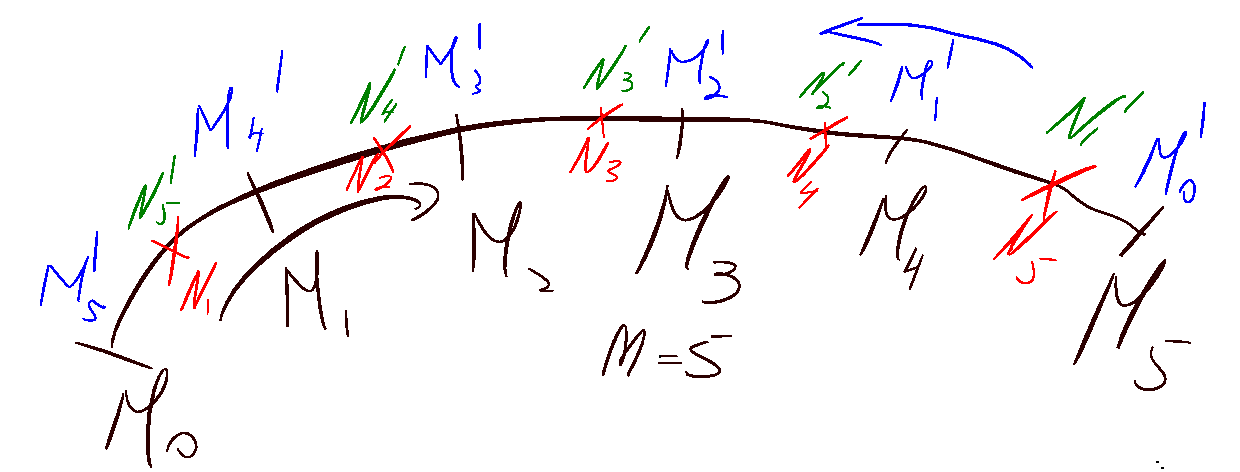
\includegraphics[width=1\linewidth]{curvilinear.pdf}
\begin{gather*}
    M^\prime_k = M_{m-k} \quad N^\prime_k = N_{m-k+1} \quad x^\prime_{kj} = x_{m-k,j}  \quad M^\prime_k= \begin{bmatrix*}
        x^\prime_{k1} \\
        \vdots \\
        x^\prime_{kn}
    \end{bmatrix*}\\
    \stackrel{\leftarrow}{\Gamma}(t) = \ldots \\ 
\end{gather*}
\begin{multline*}
    \sum^m_{k=1} f(N^\prime_k)(x^\prime_{kj} - x^\prime_{k-1,j}) = \sum^m_{k=1}f(N_m-k+1)(x_{m-k,i} - x_{m-k+1,j}) =\\
    = - \sum^m_{k=1} f(N_{m-k+1})(x_{m-k+1,j} - x_{m-k,j}) = -\sum^m_{\nu = 1}f(N_\nu) (x_{\nu j} - x_{\nu -1,j}) \tag{6}
\end{multline*}

\begin{multline*}
    S_{\stackrel{\leftarrow}{\Gamma}}(f, \{ M^\prime_k \}^m_{k=0}, \{N_k^\prime\}^m_{k=1}) = \\
    = -S_{\stackrel{\rightarrow}{\Gamma}}(f, \{ M_\nu \}^m_{\nu=0}, \{N_\nu\}_{\nu=1}^m) \tag{6\prime} \\
\end{multline*}
\[ \underset{k}{max} || M^\prime_{k-1}M^\prime_k||_{{\vR^n}} = \underset{k}{max} ||M_{m-k+1}M_{m-k}||_{{\vR^n}} =
\underset{\nu}{max} || M_{\nu-1}N_{\nu} ||_{{\vR^n}} \tag{7} \]
\begin{theorem}[Теорема о приближении криволинейного интеграла второго рода к интегральной сумме]
    \begin{gather*}
        \stackrel{\rightarrow}{\Gamma}([a,b]) \rightarrow {\vR^n} \\
        f \in C(\Gamma)\\
        \forall \varepsilon > 0 \exists \delta > 0 : \forall P = \{t_k \}^m_{k=0} |t_k - t_{k-1}| < \delta \quad 1 \leq k \leq m \\
        |S_{\stackrel{\rightarrow}{\Gamma}}(f,P,T) - \int_{\stackrel{\rightarrow}{\Gamma}} f(M)dx_j| < \varepsilon \tag{8}\\
    \end{gather*}
    $j$ у нас фиксированное, может, где-то пропустили, надо иметь это в виду
\end{theorem}
\begin{proof}
    $\delta$ выберем в конце. Сейчас будем проводить некоторые оценки, после которых будет понятно, какую $\delta$ выбрать.
    \begin{multline*}
        \underbrace{S_{\stackrel{\rightarrow}{\Gamma}}(f,P,T)}_{J} - \underbrace{\int_{\stackrel{\rightarrow}{\Gamma}}f(M)dx_j}_{I} = \sum^m_{k=1} f(\Gamma(\tau_k))(\gamma_j(t_k)-\gamma_j(t_{k-1})) - \\
        - \int^b_a f(\Gamma(t))\gamma_j^\prime(t)dt = \sum^m_{k=1}f(\Gamma(\tau_k))\int^{t_k}_{t_{k-1}} \gamma_j^\prime(t)dt - \\
        - \sum^m_{k=1} \int^{t_k}_{t_{k-1}}f(\Gamma(t))\gamma^\prime_j(t)dt = \\
        = \sum^m_{k=1} \int^{t_k}_{t_{k-1}} (f(\Gamma(\tau_k)) -f(\Gamma(t)))\gamma^\prime_j(t)dt \tag{9}
    \end{multline*}
    $f$ непрерывна на $\Gamma$, а это компакт, значит, справедлива теорема Кантора
    \begin{gather*}
        c_3 \quad \forall \tilde{M}_1, \tilde{M}_2 \in \Gamma \quad ||\tilde{M}_1\tilde{M}_2||_{{\vR^n}} < \delta_0 \implies
        |f(\tilde{M}_2 - \tilde{M}_1)| < c_3\varepsilon \tag{10}
    \end{gather*}
    Теперь хотим определить $delta_0$. Вспомним лемму между темами. Там фигурировало $c_1$ слева, $c_2$ справа
    \[ \delta : c_2\delta < \delta_0 \tag{11} \] 
    \begin{gather*}
        (10),(11) \implies t_k - t_{k-1} < \delta \forall k, \tau_k \in [t_{k-1}, t_k] \quad t \in [t_{k-1},t_k] \implies \\
        \implies |f(\Gamma(\tau_k)) - f(\Gamma(t))| < c_3 \varepsilon \tag{12}
    \end{gather*}
    \begin{multline*}
        (9)-(12) \implies |J-I| \leq \sum^m_{k=1} \left | \int^{t_k}_{t_{k-1}}(f(\Gamma(\tau_k))-f(\Gamma(t)))\gamma^\prime_j(t)dt \right | \leq \\
        \leq \sum^m_{k=1} \int^{t_k}_{t_{k-1}} |f(\Gamma(\tau_k))- f(\Gamma(t)) | |\gamma^\prime_j(t)| dt < \\
        < c_3\varepsilon \sum^{m}_{k=1} \int^{t_k}_{t_{k-1}} | \gamma_j^\prime(t)|dt = \\
        = c_3 \varepsilon \int^b_a |\gamma_j^\prime(t)|dt \leq c_3 \varepsilon \int^b_a \sqrt{(\gamma_1^\prime(t))^2+ \ldots (\gamma^\prime_n(t))^2}dt = \\
        = c_3 \varepsilon \int^b_a ||D\Gamma(t)||_{{\vR^n}}dt = c_3 \varepsilon \underbrace{L(\Gamma)}_\text{длина кривой} \tag{13} 
    \end{multline*}
    \[c_3 = \frac{1}{C(\Gamma)}\]
\end{proof}
\begin{remark}[Переформулировка теоремы]
    \begin{gather*}
        \stackrel{\rightarrow}{\Gamma} \quad f \in C(\Gamma) \quad \varepsilon > 0 \quad \exists \delta_1 > 0 : \\
        \forall \{ M_k \}^m_{k=0} \quad M_k \in \Gamma \quad ||M_{k-1}M_k||_{{\vR^n}} < \delta_1 \\
        \text{ и } \forall \{N_k \}^m_{k=1} \quad \left|S_{\stackrel{\rightarrow}{\Gamma}}(f, \{ M_k \}^m_{k=0}, \{N_k\}^m_{k=1})-
        \int_{\stackrel{\rightarrow}{\Gamma}}f(M)dx_j \right| < \varepsilon \tag{14}
    \end{gather*}
\end{remark}
\begin{proof}
    $\varepsilon$ задано. Выберем $\delta$
    \begin{gather*}
        \delta \quad P \quad |t_k - t_{k-1}| < \delta \\
        c_1 \text{ из леммы } \\
        c_1|t_k-t_{k-1}| \leq || \Gamma(\underbrace{t_k}_{M_k}) - \Gamma(\underbrace{t_{k-1}}_{M_{k-1}})||_{{\vR^n}}  \text{это Лемма}\\
        \delta_1 = c_1 \delta \\
        \text{Если } ||\Gamma(t_k) - \Gamma(t_{k-1})||_{{\vR^n}} < \delta_1 = c_1 \delta \implies \\
        \implies |t_k - t_{k-1}| < \delta
    \end{gather*}
    Это некоторая интегральная сумма с некоторыми $t_k$ и $\tau_k$ (недавно была такая теорема, потом тэгну) и в силу выбора $\delta_1$. $c_1$ из той леммы,  все доказано. 
    В формулировке (14) нет никакого $\Gamma(t)$. Следовательно, криволинейный интеграл второго рода по гладкой кривой не зависит от $\Gamma(t)$.
    По кусочно-гладкой кривой тоже.
\end{proof}

\subsection{Еще свойства криволинейных интегралов второго рода}

\begin{theorem}
    \begin{gather*}
        \stackrel{\rightarrow}{\Gamma} \text{ -- гладкая кривая} \quad f \in C(\Gamma) \\
        \stackrel{\leftarrow}{\Gamma} 
    \end{gather*}
    \[ \int_{\stackrel{\leftarrow}{\Gamma}} f(M)dx_j = - \int_{\stackrel{\rightarrow}{\Gamma}} f(M)dx_j \tag{15} \] 
\end{theorem}
\begin{proof}
    $\varepsilon > 0 \quad \delta_1$\\
    Выберем точки, чтобы они находились в соответствии с ориентацией кривой.
    \begin{gather*}
        \underbrace{\{ M_k \}^m_{k=0}}_{\stackrel{\rightarrow}{\Gamma}} \quad M_k \in \Gamma \\
        ||M_kM_{k-1}||_{{\vR^n}} < \delta_1 \\
        \forall k \\
        N_k \in \Gamma([M_{k-1},M_k])
        M^\prime_k = M_{m-k} \quad N^\prime_k = N_{m-k+1}\\
        \underbrace{\{ M^\prime_k \}^m_{k=1}}_{\stackrel{\leftarrow}{\Gamma}}\\
        S_{\stackrel{\rightarrow}{\Gamma}}(f, \{M_k\}^m_{k=1}, \{N_k\}^m_{k=1}) + 
        S_{\stackrel{\leftarrow}{\Gamma}}(f, \{M^\prime_k\}^m_{k=1}, \{N^\prime_k\}^m_{k=1}) = 0 \tag{16}
    \end{gather*}
    \begin{multline*}
        (16) = \left| \int_{\stackrel{\rightarrow}{\Gamma}}f(M)dx_j + \int_{\stackrel{\leftarrow}{\Gamma}} f(M)dx_j \right| = \\
        =  \bigg| \int_{\stackrel{\rightarrow}{\Gamma}} f(M)dx_j + \int_{\stackrel{\leftarrow}{\Gamma}} f(M)dx_j  -
        (S_{\stackrel{\rightarrow}{\Gamma}}(f, \{M_k\}, \{N_k\})) + \\ 
        + S_{\stackrel{\leftarrow}{\Gamma}}(f, \{M^\prime_k\}, \{N^\prime_k\}) \bigg| 
        \leq \varepsilon + \varepsilon = 2 \varepsilon
    \end{multline*}
    \begin{gather*}
        \left| \int_{\stackrel{\rightarrow}{\Gamma}}f(M)dx_j - S_{\stackrel{\rightarrow}{\Gamma}}(f, \{M_k\},\{N_k\}) \right| + \\
        + \left| \int_{\stackrel{\leftarrow}{\Gamma}} f(M)dx_j-S_{\stackrel{\leftarrow}{\Gamma}}(f, \{ M^\prime_k\},\{ N^\prime_k\} ) \right| \\
        || M_{k-1}M_k||_{{\vR^n}} < \delta_1 \forall k \Leftrightarrow \\
        ||M^\prime_{k-1}M^\prime_{k}||_{{\vR^n}} < \delta_1 \tag{7}\\
        < \varepsilon + \varepsilon = 2\varepsilon \implies(15)
    \end{gather*}
\end{proof}

\begin{theorem}
    \begin{gather*}
        \stackrel{\rightarrow}{\Gamma}([a,b]) \rightarrow {\vR^n} \\
        c \in \vR \Gamma(a) = \begin{bmatrix*}
            x_1^* \\
            \vdots \\
            x_n^*
        \end{bmatrix*} \quad \Gamma(b) = \begin{bmatrix}
            y_1 \\
            \vdots \\
            y_n
        \end{bmatrix} 
    \end{gather*}
    \[ \int_{\stackrel{\rightarrow}{\Gamma}}cdx_j = c(y_j - x_j^*) \]
\end{theorem}
\begin{proof}
    \begin{gather*}
        \int_{\stackrel{\rightarrow}{\Gamma}}cdx_j = \int^b_a c \gamma^\prime_j(t) = c(\gamma_j(b)-\gamma_j(a)) =
        c(y_j - x^*_j) \\
        M_k = \begin{bmatrix}
            x_{k^1} \\
            \vdots \\
            x_{k^n}
        \end{bmatrix} \quad \stackrel{\rightarrow}{\Gamma} = \bigcup^N_{k=1} \stackrel{\rightarrow}{\Gamma}_k \\
        \stackrel{\rightarrow}{\Gamma}_k \text{ начало } M_k \text{ и конец } M_{k+1} \\
        \int_{\stackrel{\rightarrow}{\Gamma}}cdx_j = \sum^m_{k=1} \int_{\stackrel{\rightarrow}{\Gamma_k}} cdx_j = \sum^N_{k=1}c(x_{k+1,j}-x_{k,j})
    \end{gather*}
\end{proof}

\begin{theorem}
    \begin{gather*}
        \stackrel{\rightarrow}{\Gamma} \quad f \in C(\Gamma) \\
        \left| \int_{\stackrel{\rightarrow}{\Gamma}} f(M) dx_j \right| \leq \int_\Gamma |f(M)|dl(M) \\
    \end{gather*}
\end{theorem}
\begin{proof}
    \begin{gather*}
        ||D\Gamma(t)||_{{\vR^n}} = \sqrt{(\gamma_1^\prime(t))^2 + \ldots + (\gamma^\prime_n(t))^2} 
    \end{gather*}
    \begin{multline*}
        \left| \int_{\stackrel{\rightarrow}{\Gamma}} f(M) dx_j \right| = \left| \int^b_a f(\Gamma(t))\gamma^\prime_j(t) dt \right| \leq\\
        \leq \int^b_a | f(\Gamma(t)) | | \gamma^\prime_j(t)| dt \leq \int^b_a |f(\Gamma(t))||D\Gamma(t)||_{\vR^n} dt = \\
        = \int_{\Gamma} f(M) dl(M) 
    \end{multline*}
    \[\stackrel{\rightarrow}{\Gamma} = \bigcup^N_{k=1} \stackrel{\rightarrow}{\Gamma}_k \] 
    \begin{multline*}
        \left| \int_{\stackrel{\rightarrow}{\Gamma}} f(M) dx_j \right| = \left| \sum^N_{k=1}
         \int_{\stackrel{\rightarrow}{\Gamma_k}} f(M)dx_j \right| \leq \sum^N_{k=1} 
         \left| \int_{\stackrel{\rightarrow}{\Gamma_k}} f(M)dx_j \right| \leq \\
         \leq \sum^N_{k=1}  \int_{Gamma_k} |f(M)|dl(M) = \int_{\Gamma} f(M)dl(M)
    \end{multline*}
    Это по определению криволинейный интеграл 1 рода
\end{proof}
\end{document}